\section{Class Diagram}

The figures below show the main classes Jadwal's system includes. The figures give an overview of interfaces in the system to help in understanding the different parts of the system. Since Golang will be used for the backend mainly, the diagrams below are more suited for it.

Of course that doesn't mean they can't be used for implementing in other languages, but the way it was written took into consideration the language features. Golang is neither fully object oriented neither fully functional. It has \texttt{interface} and \texttt{struct}, and has implicit implementation. Implicit implementation means as long as a struct has the methods that an interface expects, that struct implemented the interface. Below is a key for the class diagrams coming below:
\begin{itemize}
    \item S - \texttt{struct} (Go struct type)
    \item T - \texttt{type} (Go type definition)
    \item C - \texttt{class} (Go interface implementations)
    \item I - \texttt{interface} (Go interface definition)
\end{itemize}

\begin{figure}[!h]
    \centering
    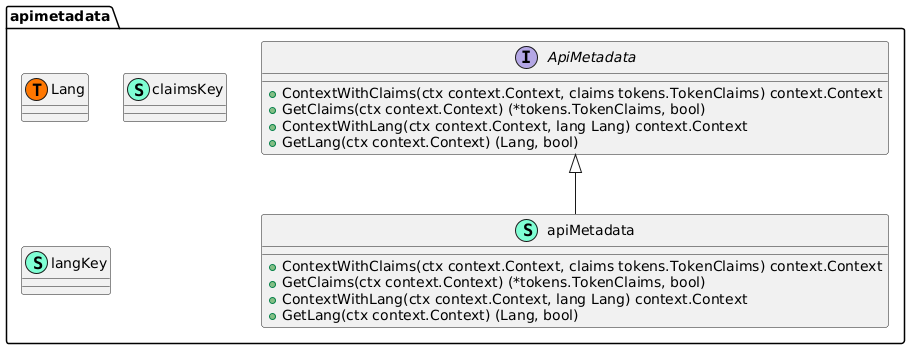
\includegraphics[width=0.9\textwidth]{images/docs/diagrams/class/class-diagram/apimetadata.png}
    \caption{Api Metadata Class Diagram}
    \label{fig:api-metadata-class-diagram}
\end{figure}

In Figure~\ref{fig:api-metadata-class-diagram}, the diagram shows the Api Metadata interface and its implementation along with important fields. It basically extracts data from the headers and includes it in the context of the requests. It helps you put stuff into the context and extract it from them. Context in Golang allows you to attach stuff to it, but it is not type safe, so we are making a wrapper to make it safe. Below we are adding wrappers for \texttt{Claims} and \texttt{Lang}. \texttt{Claims} are extracted from the JWT (JSON Web Token). \texttt{Lang} is self-explanatory.



\begin{figure}[!h]
    \centering
    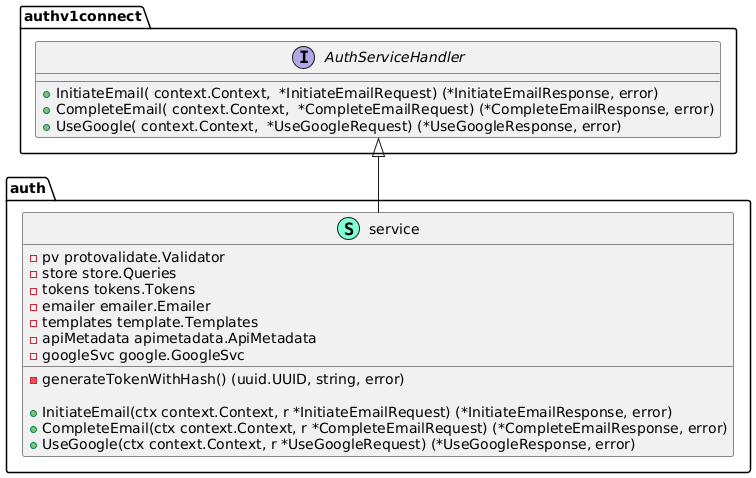
\includegraphics[width=0.9\textwidth]{images/docs/diagrams/class/class-diagram/auth.png}
    \caption{Auth Class Diagram}
    \label{fig:auth-class-diagram}
\end{figure}

In Figure~\ref{fig:auth-class-diagram}, the diagram shows the Auth API interface with its dependencies.
It also shows the \texttt{authv1connect} which is the generated code for the API\@.
This includes the flow for using email to authenticate and using Google.



\begin{figure}[!h]
    \centering
    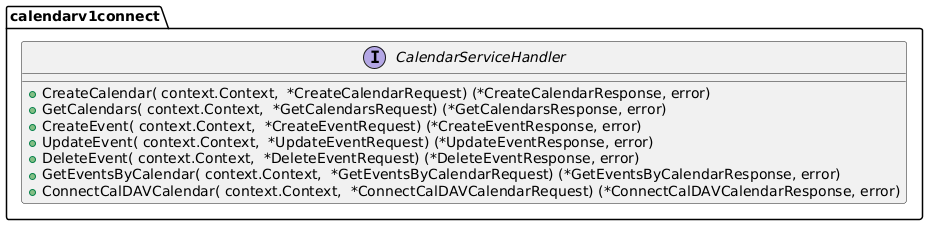
\includegraphics[width=0.9\textwidth]{images/docs/diagrams/class/class-diagram/calendarv1.png}
    \caption{Calendar V1 Class Diagram}
    \label{fig:calendar-v1-class-diagram}
\end{figure}

In Figure~\ref{fig:calendar-v1-class-diagram}, the diagram shows the api layer service calendar.
It allows Jadwal's clients to manage their calendar data easily.
It shows the interfaces and the implementation structs with their fields and methods.



\begin{figure}[!h]
    \centering
    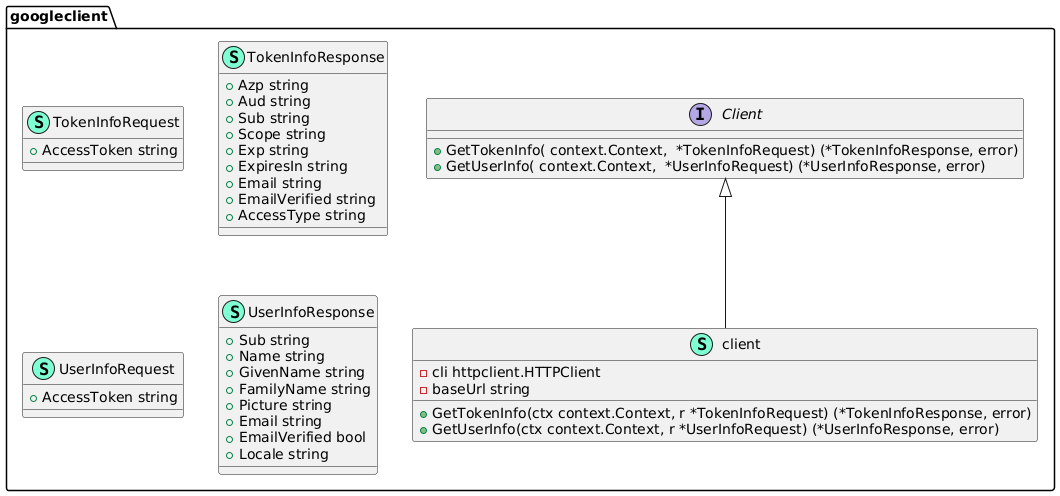
\includegraphics[width=0.9\textwidth]{images/docs/diagrams/class/class-diagram/googleclient.png}
    \caption{Google Client Class Diagram}
    \label{fig:googleclient-class-diagram}
\end{figure}

In Figure~\ref{fig:googleclient-class-diagram}, the Google client, and its methods.
It allows Jadawl to verify with Google that tokens its gets are good, and it also allows Jadwal system to get the user info the system was granted access for.



\begin{figure}[!h]
    \centering
    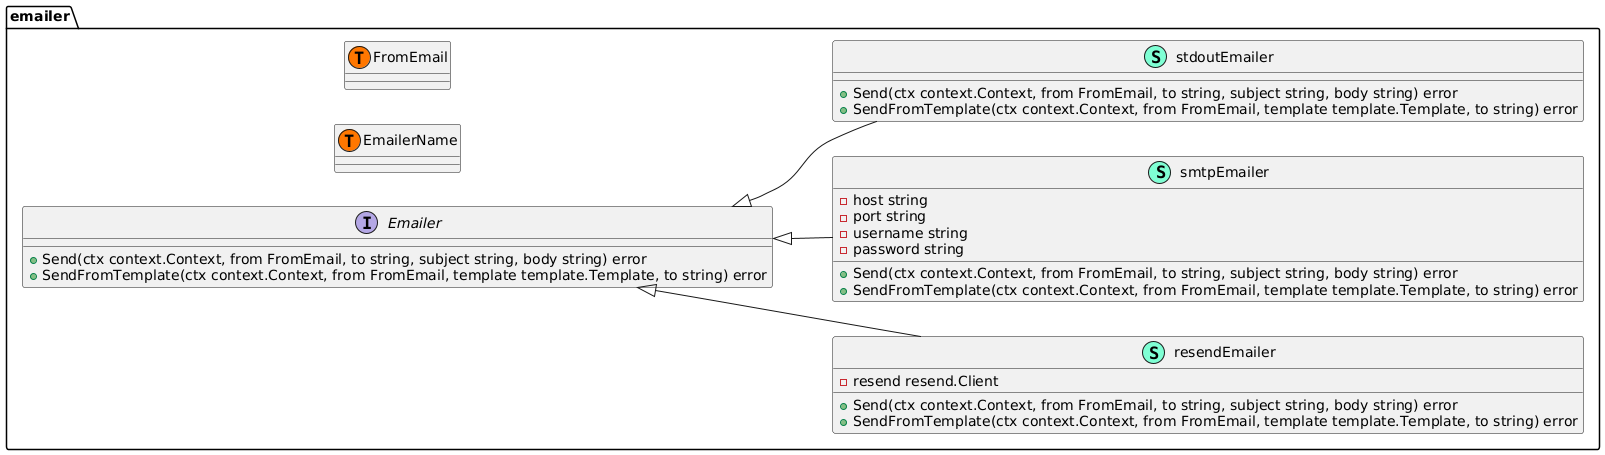
\includegraphics[width=0.9\textwidth]{images/docs/diagrams/class/class-diagram/emailer.png}
    \caption{Emailer Class Diagram}
    \label{fig:emailer-class-diagram}
\end{figure}

In Figure~\ref{fig:emailer-class-diagram}, the diagram shows the \texttt{emailer} interface with its three implementations. This allows for using the texttt{stdoutEmailer} when testing locally, and using either of the \texttt{resendEmailer} or \texttt{smtpEmailer} in production to send real emails.



\begin{figure}[!h]
    \centering
    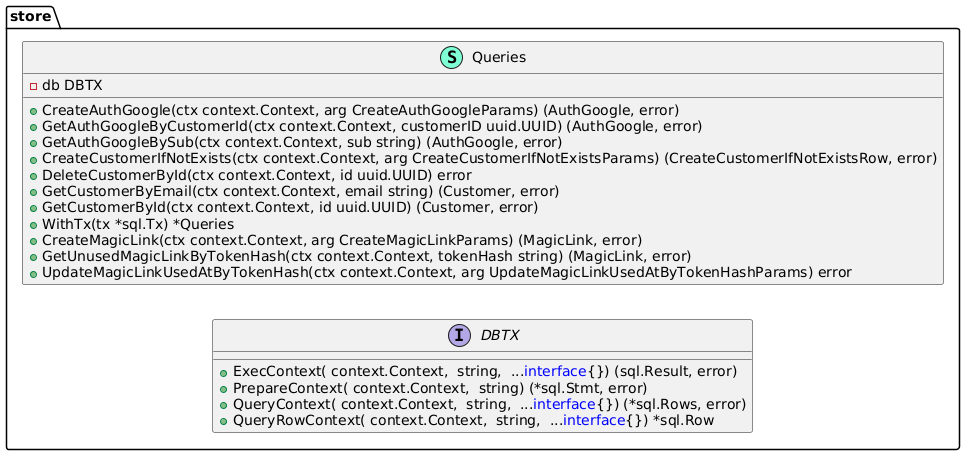
\includegraphics[width=0.9\textwidth]{images/docs/diagrams/class/class-diagram/store.png}
    \caption{Store Class Diagram}
    \label{fig:store-class-diagram}
\end{figure}

In Figure~\ref{fig:store-class-diagram}, the diagram shows the store, or in other words the database. The store holds all the methods needed to query the database for information it holds. More methods can be added as needed, but those are the core methods.



\begin{figure}[!h]
    \centering
    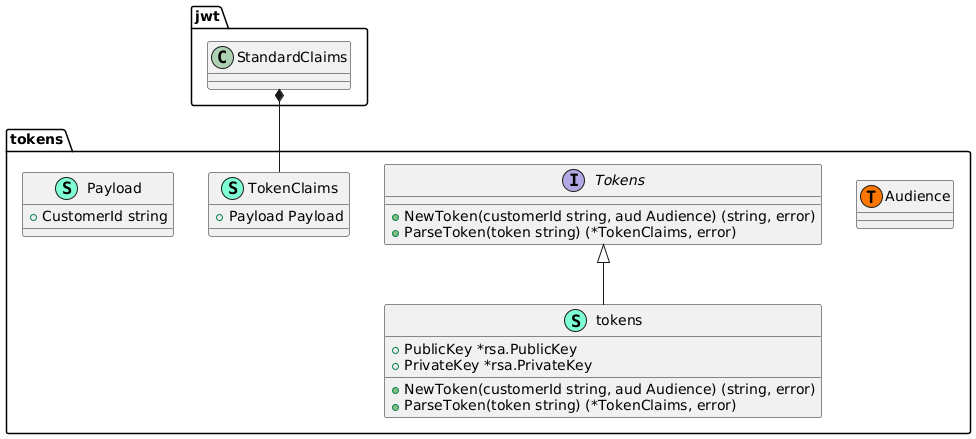
\includegraphics[width=0.9\textwidth]{images/docs/diagrams/class/class-diagram/tokens.png}
    \caption{Tokens Class Diagram}
    \label{fig:tokens-class-diagram}
\end{figure}

In Figure~\ref{fig:tokens-class-diagram}, the diagram shows the tokens service implementation along with its interface. The diagram also illustartes the needed \texttt{struct} representation for any data passed to and from the service.



\begin{figure}[!h]
    \centering
    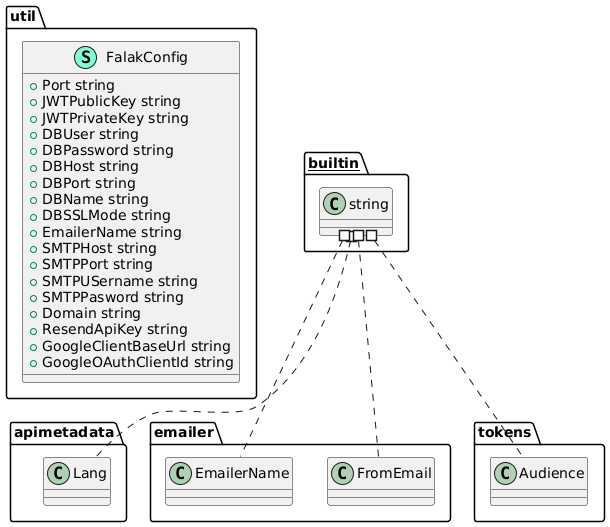
\includegraphics[width=0.5\textwidth]{images/docs/diagrams/class/class-diagram/util.png}
    \caption{Util Class Diagram}
    \label{fig:util-class-diagram}
\end{figure}

In Figure~\ref{fig:util-class-diagram}, the diagram shows config needed to support both production and development without committing secrets to the codebase. Falak in this context is the codename for the backend. The config here is represented as a \texttt{struct} since it is hold data and doesn't need implementations.